\section{Ergebnis} % (fold)
\label{sec:ergebnis}
	Bereits zu Beginn des Projekts war es wichtig es messbar zu machen. Dafür wurde eine Testumgebung aufgebaut, mit deren Hilfe die Seite nach ihrer Geschwindigkeit getestet werden kann. Ganz entscheidend war dabei die Webpagetest API in Verbindung mit Google Spreadsheets. Damit lassen sich regelmäßig automatisierte Tests durchführen und die Daten werden nach erfolgreichem Test automatisch in einer Spreadsheet Tabelle gespeichert. Die über den Zeitraum der Arbeit hinweig gesammelten Daten sind hier finden: \url{http://tinyurl.com/l5usz79}. Diese Daten wurden anschließend mittels \url{http://Chartjs.org} in Diagrammen aufbereitet und alle Diagramme sind auch Online abrufbar unter: \url{http://bithugger.github.io/bachelorthesis/}

	\subsection{Wie wurde getestet?} % (fold)
	\label{sub:wie_wurde_getestet}
		Damit mittels Google Spreadsheets die Webpagetest API verwendet werden kann, ist es nötig einen sogenannten API-Key anzufordern. Ein solcher Key ist kostenlos unter der Adresse: \url{http://www.webpagetest.org/getkey.php} zu erhalten und bietet die Möglichkeit täglich 200 Seitenaufrufe zu tätigen. Als Seitenaufruf zählt sowohl die "`first view"' als auch "`repeat view"'. Die Tests sind 30 Tage abrufbar und gespeichert.\\

		Für das Testen der Seite kann aus einer Vielzahl an Teststandorten gewählt werden. Damit lässt sich nachvollziehen wie beispielsweise die Ladezeiten aus der USA oder Asien sind. Je nach Zielgruppe sollten Tests von verschiedenen Standorten in betracht gezogen werden.\footnote{Eine volle Liste der zur Verfügung stehenden Teststandorte ist im Anhang unter Punkt: \ref{sub:webpagetest_teststandorte} zu finden.} Für dieses Projekt wurden ausschließlich Teststandorte aus der USA und Europa gewählt.\\

		Als Testparameter wurde eine Anzahl von 9 Tests pro Testlauf gewählt. Dabei wurde sowohl die "`first view"' als auch die "`repeat view"' aufgezeichnet. Von den 9 Testläufen wurde der Median als Ergebnis des Testlaufs verwendet. Über den Zeitraum der Arbeit wurde die Seite 1089 Tests unterzogen.\\

		Das größte Problem bestand in der möglichst genauen Messzeiterfassung für die Ladezeiten mittels Smartphone. Webpagetest stellt nur einen Smartphones Teststandort in Dulles USA zu Verfügung. Da die Latenz zwischen dem Hosting in Deutschland und dem Seitenaufruf in der USA sehr viel größer ist, als wenn dieser direkt aus Deutschland erfolgt, wurde nach einer Lösung gesucht diese Messungen exakter zu gestalten.
		Die Lösung dafür ist, ein zweites Hosting mit der selben Seite in den USA zu erstellen. Dafür wurde die "`Microsoft Azure Cloud"' verwendet. Eine kostenlose Testversion ermöglicht es, ganz einfach auf verschiedensten Kontinenten eine Webseite zu hosten. Die Seite wurde für die Tests Online geschaltet und nach den Testläufen wieder Offline genommen.

	% subsection wie_wurde_getestet (end)

	\subsection{Datenauswertung}
	\label{sub:datenauswertung}
		Folgende Daten wurden bei jedem Testlauf erfasst:

		\begin{itemize}
			\item Speed Index
			\item TTFB (ms)
			\item Render start (ms)
			\item Visually complete (ms)
			\item Dom Content loaded (ms)
			\item Site fully loaded (ms)
			\item Requests
			\item Bytes in Document
		\end{itemize}

        Das Diagramm in Abbildung \ref{fig:data_all}, zeigt eine Übersicht der verschiedenen Messwerte über den Zeitraum des Projekts. Die Y-Achse bildet die Zeit in Millisekunden ab und die X-Achse ist das Datum der Messung. Innerhalb von 36 Tagen haben sich alle Werte signifikant verbessert.
        % todo: wirklich 36 Tage? Nachzählen!

        \begin{itemize}
            \item Speed Index: Ein Speed Index von < 1000 Punkten wird als "`schnell genug"' angesehen. Der Median des Speed Indexes konnte von 6063 Zählern auf 1028 Zähler verringert werden. Ein niedriger Speed Index zeugt von der beachtung der \texttt{best practices}, denn er berechnet sich aus einer vielzahl von Faktoren. 
            % welche vielzahl an faktoren?
            % todo, evt Zitat von Twittter (how fast is fast enough?)
            % fazit: was bedeutet der Speed Index jetzt konkret für den Anwender / Nutzer / fürs Projekt?
            % todo, evt vergleich mit speed index der top 1000 Alexa sites
            \item Render Start: Während dieser Wert bereits bei Projektbeginn mit 2,4 Sekunden für das erste Rendern recht gut war, konnte auch hier fast das dreifache der Zeit (287\%) eingespart werden. Dieser Wert wird durch dieses Diagramm nicht drastisch genug ausgedrückt. So konnte die alte Version der Seite auf dem Smartphone durchaus einen \texttt{Render start} von ganzen 10 Sekunden haben. Das dieser Wert im Diagramm vergleichbar gering ausfällt liegt daran, dass auch viele Tests mittels Desktop PC und Kabelverbindung eingeflossen sind. Die jetzige Renderzeit auf dem Smartphone beträgt ungefähr 1,4 Sekunden. 
            % note: daten, die den render start von 1,4 sec belegen?
            \item Die Ladezeit bestimmt, wie lange ein Anwender warten muss, bis eine Interaktion mit der Seite möglich ist. Dieser Wert konnte um volle 2 Sekunden verringert werden.
            % nachprüfen ob das mit der Interaktionszeit so stimmt
            \item Visually Complete: Der höchste Messwert mit rund 7,6 Sekunden konnte auf 1,2 Sekunden verringert werden. Der Hauptgrund dafür ist die Priorisierung des Inhalts "`above the fold"'. Bei der alten Version erfolge keine priorisierung, welche Bilder zuerst und welche zuletzt geladen werden sollen. Dadurch konnte es sein, dass Bilder die sehr weit unten platziert waren, zuerst geladen wurden. In der neuen Version wird alles, was unterhalb des "`above the fold"' ist verzögert geladen.
            \item TTFB: Dieser Wert ist grundsätzlich durch eine Verbesserung des Hostings gesunken. 
        \end{itemize}

		\begin{figure}[htbp]
			\begin{center}
				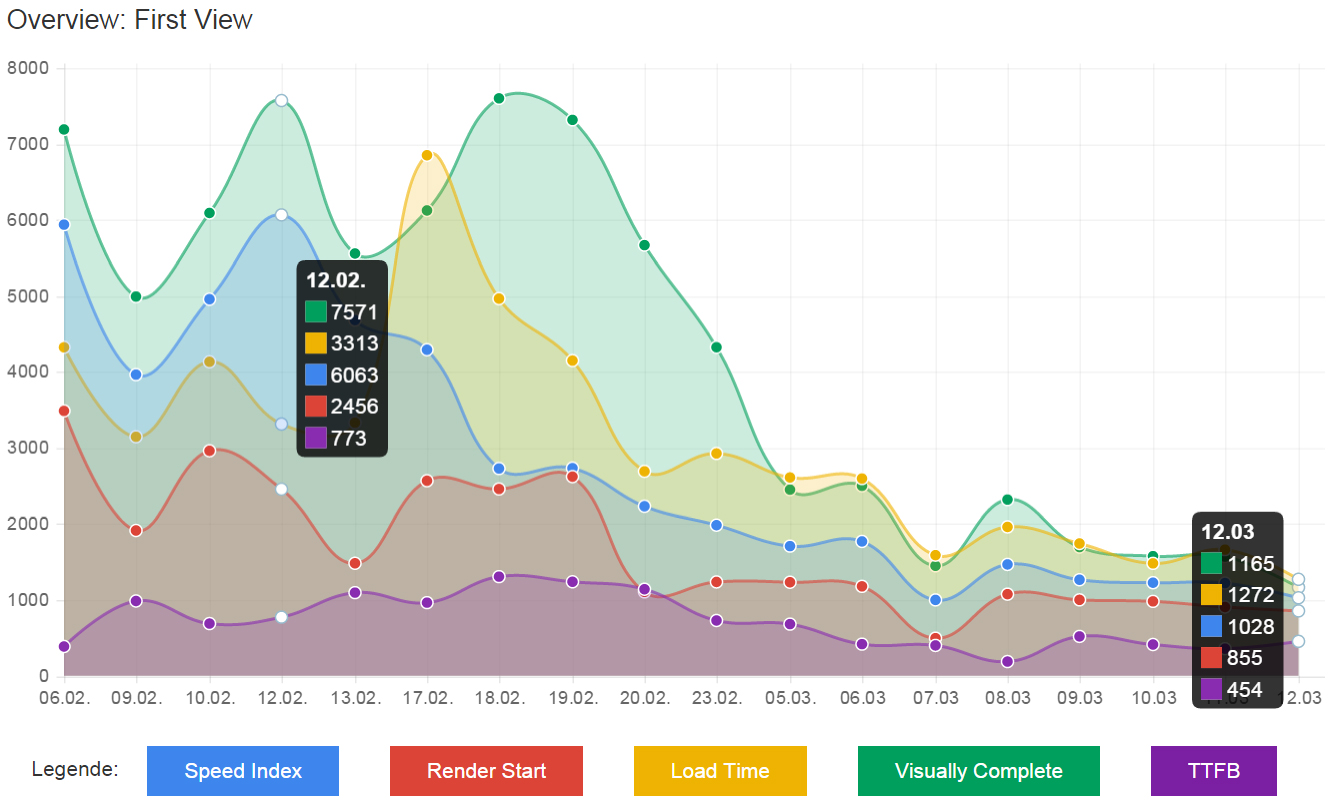
\includegraphics[width=\textwidth]{data_all.jpg}
				\caption{Datenauswertung - Überblick }
				\label{fig:data_all}
			\end{center}
		\end{figure}

		\begin{figure}[htbp]
			\begin{center}
				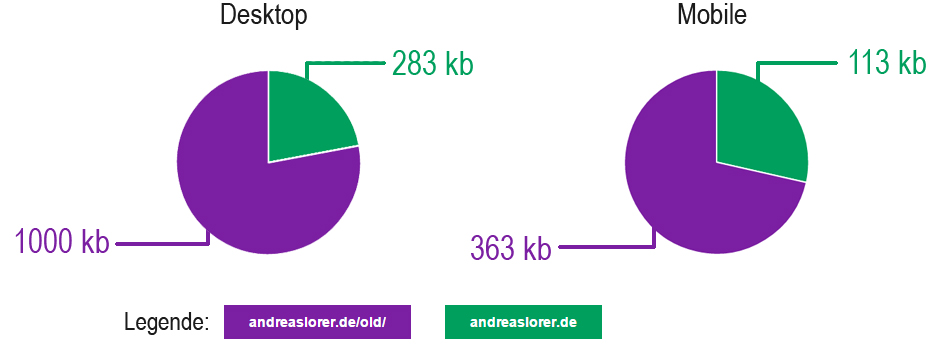
\includegraphics[width=\textwidth]{site_size_in_kb.jpg}
				\caption{Seitengröße in Kilobyte}
				\label{fig:site_size_in_kb}
			\end{center}
		\end{figure}

		\begin{figure}[htbp]
			\begin{center}
				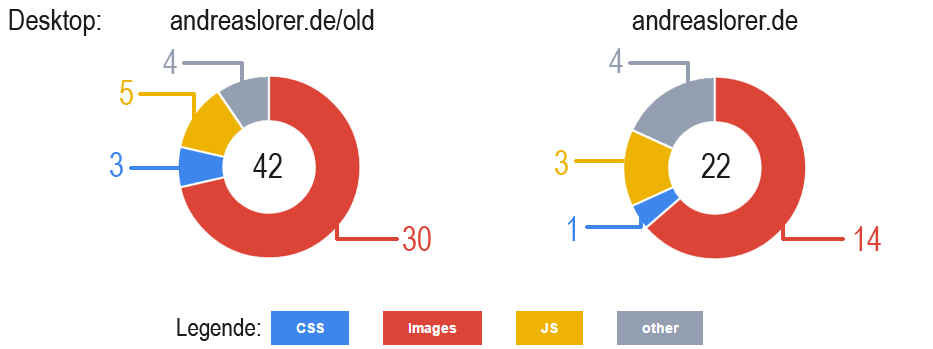
\includegraphics[width=\textwidth]{amount_of_requests.jpg}
				\caption{Anzahl an Requests via Desktop}
				\label{fig:amount_of_requests}
			\end{center}
		\end{figure}	

		\begin{figure}[htbp]
			\begin{center}
				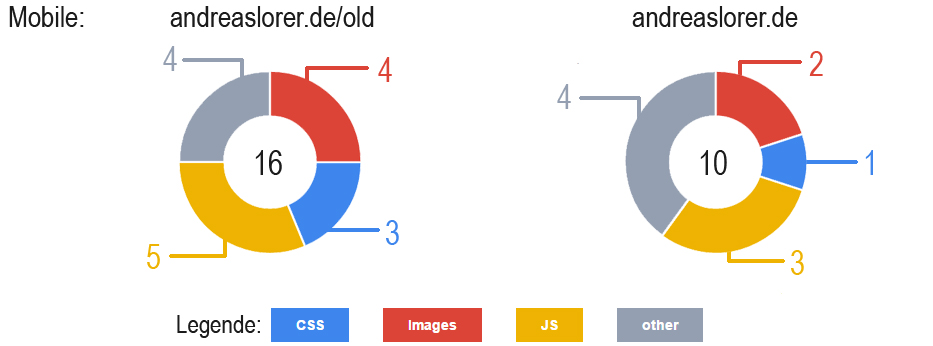
\includegraphics[width=\textwidth]{amount_of_requests_mobile.jpg}
				\caption{Anzahl an Requests via Mobile}
				\label{fig:amount_of_requests_mobile}
			\end{center}
        \end{figure}
			
				

	% subsection datenauswertung (end)
% section ergebnis (end)

\pagebreak
